%%%%%%%%%%%%%%%%%%%%%%%%%%%%%%%%%%%%%%%%%%%%%%%%%%%
%% P3: Phenomenology of Particle Physics                         
%%
%% Author:  André Rubbia                   		 
%%
%% Figure 12.6 Basic illustration of the vacuum polarization effect inducing the ``running'' of the coupling constant $\alpha$.
%%
%% This work is licensed under the Creative Commons Attribution 4.0 International License. 
%% To view a copy of this license, visit http://creativecommons.org/licenses/by/4.0/ or 
%% send a letter to Creative Commons, PO Box 1866, Mountain View, CA 94042, USA.
%%
%%%%%%%%%%%%%%%%%%%%%%%%%%%%%%%%%%%%%%%%%%%%%%%%%%%

\documentclass[a4paper,10pt]{article}

\usepackage[T1]{fontenc}
\usepackage[utf8]{inputenc}
\usepackage{lmodern}
\usepackage[labelfont=bf]{caption}
\usepackage{upgreek}

\usepackage{tikz}
\usepackage{pgfplots}
\pgfplotsset{compat=1.17}
\usepgfplotslibrary{ternary}
\usepgfplotslibrary{fillbetween}
\usepgfplotslibrary{external}

\usepackage{braket}

\def\d{\mathrm{d}}

\begin{document}

%%%%%%%%%%%%%%%%% FIGURE %%%%%%%%%%%%%%%%%%%%%%%%%%%%%%%%%%
\begin{figure}[htb]
\begin{center}
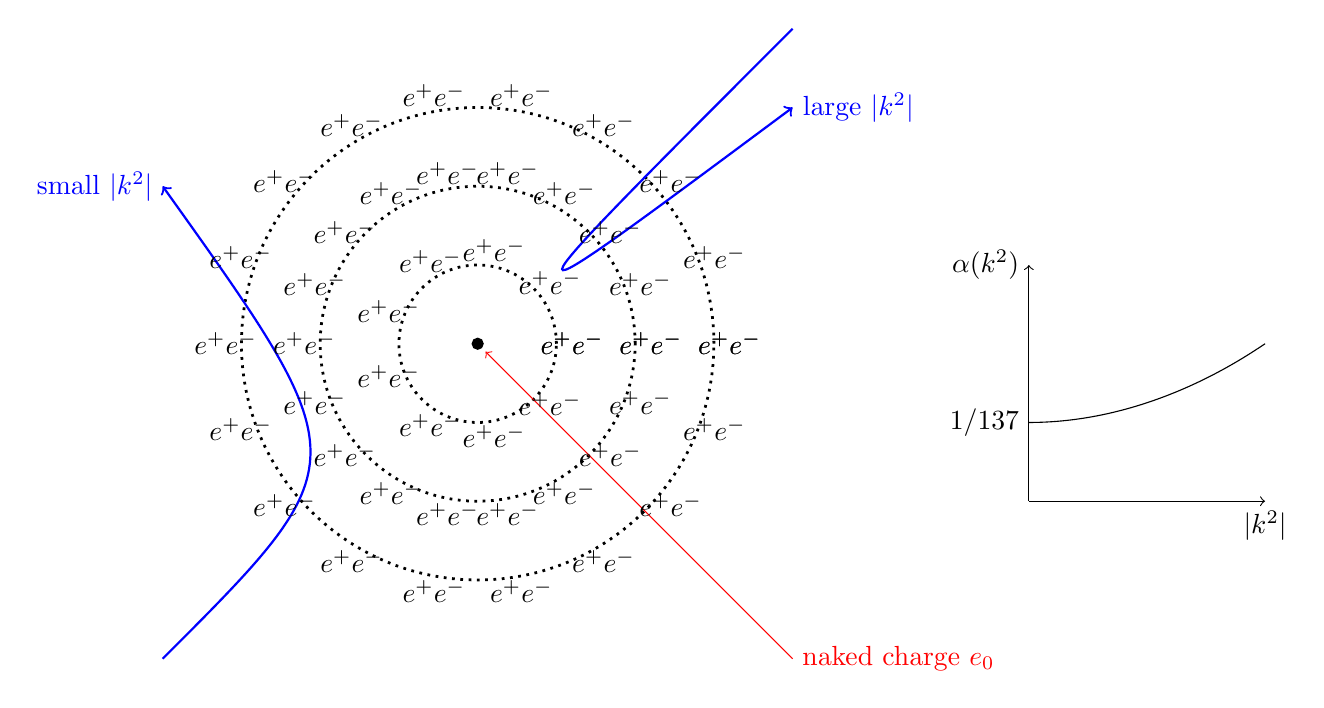
\begin{tikzpicture}
\filldraw [black] (0,0) circle (2pt);
\draw[dotted,line width=1pt] (0,0) circle (1cm);
\draw[dotted,line width=1pt] (0,0) circle (2cm);
\draw[dotted,line width=1pt] (0,0) circle (3cm);
\draw[blue,thick,->] (-4,-4) .. controls (-1.5,-1.5) .. (-4,2) node[left] {small $|k^2|$};
\draw[blue,thick,->] (4,4) .. controls (0.1,0.1) .. (4,3) node[right] {large $|k^2|$};
\draw[->,red] (4,-4) node[right] {naked charge $e_0$} -- (0.1,-0.1);
\foreach \x in {0,...,18}
    \draw (0,0) +(\x*20:3.2) node {$e^+e^-$};
\foreach \x in {0,...,18}
    \draw (0,0) +(\x*20:2.2) node {$e^+e^-$};
\foreach \x in {0,...,9}
    \draw (0,0) +(\x*40:1.2) node {$e^+e^-$};
\draw[->] (7,-2) -- (10,-2) node[below] {$|k^2|$};
\draw[->] (7,-2) -- (7,1) node [left] {$\alpha(k^2)$};
\draw (7,-1) node[left] {$1/137$} parabola (10,0);
\end{tikzpicture}
\caption{Basic illustration of the vacuum polarization effect inducing the ``running'' of the coupling constant $\alpha$.}
\end{center}
\end{figure}
%%%%%%%%%%%%%%%%% END FIGURE %%%%%%%%%%%%%%%%%%%%%%%%%%%%%%
%

\end{document}
